%%%%%%%%%%%%%%%%%%%%%%%%%%%%%%%%%%%%%%%%%%%%%%%%%%%%%%%%%%%% 
% Name: XeTeX+xeCJK日常使用模板
% Author: Lox Freeman
% Email: xiaohanyu1988@gmail.com
% 、
% 本文档可以自由转载、修改,希望能给广大TeXer的中文之路提供一些方便。
%%%%%%%%%%%%%%%%%%%%%%%%%%%%%%%%%%%%%%%%%%%%%%%%%%%%%%%%%%%% 

\documentclass[a4paper, 12pt, titlepage]{article}

%%%%%%%%%%%%%%%%%%%%%%%%% xeCJK相关宏包%%%%%%%%%%%%%%%%%%%%%%%%%
\usepackage{xltxtra,fontspec,xunicode}
\usepackage[slantfont, boldfont, CJKchecksingle]{xeCJK}

\CJKsetecglue{\hskip 0.15em plus 0.05em minus 0.05em}
% slanfont: 允许斜体
% boldfont: 允许粗体
% CJKnormalspaces: 仅忽略汉字之间的空白,但保留中英文之间的空白。
% CJKchecksingle: 避免单个汉字单独占一行。
% CJKaddspaces: [备选]忽略汉字之间的空白,并且自动在中英文转换时插入空白。

% \CJKlanguage{zh-cn}                 % 中文标点特殊处理
\XeTeXlinebreaklocale "zh"           % 针对中文进行断行
\XeTeXlinebreakskip = 0pt plus 1pt minus 0.1pt
% 给予TeX断行一定自由度
%%%%%%%%%%%%%%%%%%%%%%%%% xeCJK%%%%%%%%%%%%%%%%%%%%%%%%%%%%%%%%

%%%%%%%%%%%%% 日常所用宏包、通通放在一起%%%%%%%%%%%%%%%%%%%%%%%%%%%%
% 什么常用的宏包都可以放这里。下面是我常用的宏包,每个都给出了简要注释
\usepackage[top=2.5cm, bottom=3cm, left=2.5cm, right=2.5cm]{geometry} % 控制页边距
\usepackage{enumerate}               % 控制项目列表
\usepackage{multicol}                % 多栏显示

\usepackage[%
pdfstartview=FitH,%
CJKbookmarks=true,%
bookmarks=true,%
bookmarksnumbered=true,%
bookmarksopen=true,%
colorlinks=true,%
citecolor=seco,%
linkcolor=seco,%
anchorcolor=seco,%
urlcolor=seco%
]{hyperref}                          % 超链接相关设置

\usepackage{titlesec}                % 控制标题
\usepackage{titletoc}                % 控制目录
\usepackage{type1cm}                 % 控制字体大小
\usepackage{indentfirst}             % 首行缩进,用\noindent取消某段缩进
\usepackage{bbding}                  % 一些特殊符号
\usepackage{cite}                    % 支持引用
\usepackage{framed,color,xcolor}     % 支持彩色文本、底色、文本框等
\usepackage{latexsym}                % LaTeX一些特殊符号宏包
\usepackage{amsmath}                 % AMS LaTeX宏包
\usepackage{bm}                      % 数学公式中的黑斜体
\usepackage{relsize}                 % 调整公式字体大小:\mathsmaller, \mathlarger
\usepackage{soul}                    % 下划线自动回车换行
\usepackage{attachfile}              % 添加附见使用的宏包
\usepackage{parcolumns}              % 列排版
\usepackage{framed}
\usepackage{tcolorbox}
\usepackage{pdfpages}                % 直接引用已有的PDF文件
\usepackage{soul}                    % 自动换行的下划线
\makeindex                           % 生成索引

\makeatletter
\let\std@footnotetext\@footnotetext
\usepackage{setspace}
\let\@footnotetext\std@footnotetext
\makeatother

%%%%%%%%%%%%%%%%%%%%%%%%% 绘图方法%%%%%%%%%%%%%%%%%%%%%%%%%%%
\usepackage{graphicx}                % 图形宏包
\graphicspath{{./figure/}{./figures/}{./image/}{./graphics/}{./graphic/}{./pictures/}{./picture/}}

\usepackage{tikz}
\usepackage{amsmath,bm,times}
\usepackage{verbatim}

\usepackage{tabularx}

\usetikzlibrary{shapes,arrows,shadows,fit,snakes,positioning,decorations}
\usetikzlibrary{decorations.shapes}
\usetikzlibrary{calc}           %coordinate

\usepackage{caption}
\usepackage{float}

\ifx\du\undefined
\newlength{\du}
\fi
\setlength{\du}{15\unitlength}

\newlength\Textwd
\setlength\Textwd{3cm}
\newcommand\Textbox[2]{%
  \parbox[c][#1][c]{\Textwd}{\linespread{0.5}\centering#2}}

\makeatletter
\DeclareRobustCommand{\rvdots}{%
  \vbox{
    \baselineskip6\p@\lineskiplimit\z@
    \kern-\p@
    \hbox{.}\hbox{.}\hbox{.}
  }}
\makeatother


\makeatletter
\DeclareRobustCommand{\rvdots}{%
  \vbox{
    \baselineskip4\p@\lineskiplimit\z@
    \kern-\p@
    \hbox{.}\hbox{.}\hbox{.}}}
\tikzset{
  heights/.code={
    \def\pgf@tempb{}%
    \foreach \qrr@tikz@rs@height[count=\qrr@tikz@count from 1] in {#1}{
      \edef\pgf@tempa{\noexpand\pgfkeysalso{/tikz/every \pgf@lib@sh@toalpha\qrr@tikz@count\space node part/.append style={height={\qrr@tikz@rs@height}}}}%
      \ifnum\qrr@tikz@count=1\relax % allows to use \nodepart{text} (or not at all for the first part)
      \edef\pgf@tempa{\unexpanded\expandafter{\pgf@tempa}\noexpand\pgfkeysalso{/tikz/every text node part/.append style={height={\qrr@tikz@rs@height}}}}%
      \fi
      \expandafter\pgfutil@g@addto@macro\expandafter\pgf@tempb\expandafter{\pgf@tempa}
    }
    \pgf@tempb
  },
  height/.code={%
    \expandafter\def\expandafter\pgfutil@minipage\expandafter[\expandafter##\expandafter 1\expandafter]\expandafter{\pgfutil@minipage[][#1][c]}% LaTeX only!
  }
}

\makeatother
\tikzset{rect/.style={
    draw,
    rectangle split,
    rectangle split parts=1,
    rectangle split part align=center,
    draw,
    % font=\ttfamily, % still works
    thick,
    text width=2.5cm,
    align=center,
    rectangle split part align={center,left,right},
    % rectangle split part fill={PaleTurquoise1},
  }}

\makeatletter
\newcommand{\gettikzxy}[3]{%
  \tikz@scan@one@point\pgfutil@firstofone#1\relax
  \edef#2{\the\pgf@x}%
  \edef#3{\the\pgf@y}%
}
\makeatother
%%%%%%%%%%%%%%%%%%%%%%%%% 绘图方法结束%%%%%%%%%%%%%%%%%%%%%%%%%%%

%%%%%%%%%%%%%%%%%%%%%%%%% fancyhdr设置页眉页脚%%%%%%%%%%%%%%%%%%%%
\usepackage{etoolbox}
\usepackage{fancyhdr}                % 页眉页脚
\pagestyle{fancy}                    % 页眉页脚风格
\setlength{\headheight}{15pt}        % 有时会出现\headheight too small的warning

\makeatletter
\patchcmd{\@fancyhead}{\rlap}{\color{seco}\rlap}{}{}
\patchcmd{\headrule}{\hrule}{\color{seco}\hrule}{}{}
\patchcmd{\@fancyfoot}{\rlap}{\color{seco}\rlap}{}{}
\patchcmd{\footrule}{\hrule}{\color{seco}\hrule}{}{}
\makeatother
%%%%%%%%%%%%%%%%%%%%%%%%% fancyhdr设置结束%%%%%%%%%%%%%%%%%%%%%%%

%%%%%%%%%%%%%%%%%%%%%%%%% xeCJK字体设置%%%%%%%%%%%%%%%%%%%%%%%%%
% \setmainfont[Ligatures=TeX]{Minion Pro} % (\textrm)
\setmainfont[Ligatures=TeX]{Calibri} % (\textrm)
% \setsansfont{Myriad Pro}                % (\textsf)
\setsansfont{Calibri}                % (\textsf)
% \setmonofont{Adobe Garamond Pro}        % Palatino Linotype
\setmonofont{Ubuntu Mono}        % Palatino Linotype

\setCJKmainfont[BoldFont={方正兰亭纤黑_GBK},ItalicFont={Adobe Kaiti Std}]{Adobe Kaiti Std}
\setCJKsansfont[BoldFont={方正兰亭纤黑_GBK}]{方正兰亭纤黑_GBK}
\setCJKmonofont{方正兰亭纤黑_GBK}
%%%%%%%%%%%%%%%%%%%%%%%%% xeCJK字体设置结束%%%%%%%%%%%%%%%%%%%%%%

%%%%%%%%%%%%%%%%%%%%%%%%% listings宏包粘贴源码%%%%%%%%%%%%%%%%%%%%
\usepackage{listings}                % 方便粘贴源代码,部分代码高亮功能
\lstloadlanguages{}                  % 所要粘贴代码的编程语言

\newfontfamily\listingsfont{Ubuntu Mono}
\newfontfamily\listingsfontinline{Calibri}

\definecolor{sh_keyword}{rgb}{0.06, 0.10, 0.98}   % #101AF9
\definecolor{shadecolor}{rgb}{0.83, 0.83, 0.83}
\definecolor{monokai-grey-dark}{RGB}{39, 40, 34}   % #272822
\definecolor{monokai-yellow-light}{RGB}{248, 248, 246}   % #F8F8F2
\definecolor{monokai-green}{RGB}{166, 226, 42}
\definecolor{dark green}{rgb}{0.000000,0.392157,0.000000}
\definecolor{forest green}{rgb}{0.133333,0.545098,0.133333}
\def\lstsmallmath{\leavevmode\ifmmode \scriptstyle \else  \fi}
\def\lstsmallmathend{\leavevmode\ifmmode  \else  \fi}

% \definecolor{seco}{RGB}{9,80,3}
% \definecolor{seco}{RGB}{0,145,215}
\definecolor{seco}{RGB}{0,175,152}
\definecolor{main}{RGB}{127,191,51}

% \makeatletter
%   \newcommand\listingfont{\@setfontsize\listingfont{11pt}{13.2pt}}
% \makeatother

\renewcommand{\lstlistingname}{代码}

\lstset {
  language=c++,
  backgroundcolor=\color{monokai-grey-dark},
  % frame=shadowbox,
  % breaklines,
  % rulesepcolor=\color{red!20!green!20!blue!20},
  showspaces=false,showtabs=false,tabsize=4,
  numberstyle=\tiny\color{black},numbers=left,
  % basicstyle= \listingfont\listingsfont\color{monokai-yellow-light},
  basicstyle= \small\listingsfont\color{monokai-yellow-light},
  stringstyle=\color{dark green},
  % keywordstyle = \color{monokai-green}\bfseries,
  keywordstyle = \color{monokai-green},
  commentstyle=\footnotesize\color{forest green}\itshape,
  captionpos=b,
  showspaces=false,showtabs=false, showstringspaces=false,
  xleftmargin=0.7cm, xrightmargin=0.5cm,
  % lineskip=-0.3em,
  breaklines=tr,
  escapebegin={\lstsmallmath}, escapeend={\lstsmallmathend},
  extendedchars=false
}

\lstnewenvironment{acol}[1][]{\lstset{language={[x86masm]Assembler},#1}}{}
\newenvironment{parcolumenv}[1] {\begin{spacing}{#1}}{\end{spacing}}
%%%%%%%%%%%%%%%%%%%%%%%%% listings宏包设置结束%%%%%%%%%%%%%%%%%%%%


%%%%%%%%%%%%%%%%%%%%%%%%% 一些关于中文文档的重定义%%%%%%%%%%%%%%%%%

%%%% 数学公式定理的重定义%%%%
\newtheorem{example}{例}                                   % 整体编号
\newtheorem{algorithm}{算法}
\newtheorem{theorem}{定理}[section]                        % 按 section 编号
\newtheorem{definition}{定义}
\newtheorem{axiom}{公理}
\newtheorem{property}{性质}
\newtheorem{proposition}{命题}
\newtheorem{lemma}{引理}
\newtheorem{corollary}{推论}
\newtheorem{remark}{注解}
\newtheorem{condition}{条件}
\newtheorem{conclusion}{结论}
\newtheorem{assumption}{假设}

%%%% 章节等名称重定义%%%%
\renewcommand{\contentsname}{目\hspace{2em}录}
\renewcommand{\indexname}{索引}
\renewcommand{\listfigurename}{插图目录}
\renewcommand{\listtablename}{表格目录}
\renewcommand{\figurename}{图}
\renewcommand{\tablename}{表}
\renewcommand{\appendixname}{附\hspace{2em}录}

%%%% 设置chapter、section与subsection的格式%%%%
\titleformat{\chapter}{\centering\huge}{\color{seco}第\thechapter{}章}{1em}{\color{seco}\textbf}
\titleformat{\section}{\centering\LARGE}{\color{seco}\thesection}{1em}{\color{seco}\textbf}
\titleformat{\subsection}{\Large}{\color{seco}\thesubsection}{1em}{\color{seco}\textbf}
%%%%%%%%%%%%%%%%%%%%%%%%% 中文重定义结束%%%%%%%%%%%%%%%%%%%%


%%%%%%%%%%%%%%%%%%%%%%%%% 一些个性设置%%%%%%%%%%%%%%%%%%%%%%
\setlength{\parskip}{0.5\baselineskip}     % 设定段间距
\linespread{1.6}                           % 设定行距
\newcommand{\pozhehao}{\kern0.3ex\rule[0.8ex]{2em}{0.1ex}\kern0.3ex}% 中文破折号,据说来自清华模板

\setCJKfamilyfont{title}{方正正中黑简体}

\newcommand*{\TitleFont}{\usefont{\encodingdefault}{\rmdefault}{b}{n}\fontsize{32}{40}\selectfont\CJKfamily{title}\color{seco}}% 标题字体设置

\renewcommand{\today}{\color{seco}\number\year 年 \number\month 月 \number\day 日}
%%%%%%%%%%%%%%%%%%%%%%%%% 个性设置结束%%%%%%%%%%%%%%%%%%%%%%


%%%%%%%%%%%%%%%%%%%%%%%%% 正文部分%%%%%%%%%%%%%%%%%%%%%%%%%
\begin{document}
\setlength{\parindent}{2em}
% 设定首行缩进为2em。注意此设置一定要在document环境之中。
% 这可能与\setlength作用范围相关

\title{\TitleFont 数组初始化--memset or \{0\}\vspace{8cm}}
\author{\href{mailto:q00148943@gmail.com}{\LARGE{秦新良}}}
\date{\vspace{0.5cm}\today}

\maketitle

\tableofcontents
\newpage
\section{缘起}
平时在编码或代码检视的时候,有时候会听到这样的说法:数组初始化直接用\{0\},不要调用memset,这样执行效率高,如代码\ref{lst1}所示。
\begin{spacing}{1.0}
\lstinputlisting[label=lst1,caption=\{0\}初始化]{list/array.c}
\end{spacing}
但有时候又会听到截然不同的另外一种说法:数组初始化用memset,这样比直接用\{0\}初始化效率高很多,如代码\ref{lst2}所示。
\begin{spacing}{1.0}
\lstinputlisting[label=lst2,caption=memset初始化]{list/memset.c}
\end{spacing}


当只有一种观点的时候,一般会相信其的正确性\footnote{因为自己不清楚,既然有人清楚是怎么回事,也就相信是这么回事了。}。但当两种完全相反的观点同时存在时,不得不上人对孰是孰非产生一个大大的疑问,所以就有了把两种代码编译后的结果分析一下的想法。

\section{从汇编说起}
\subsection{环境信息}
本文实验所用的环境为Linux + GCC,如图\ref{fig1}所示。
\begin{figure}[!htb]
  \setlength{\abovecaptionskip}{0pt}
  % \setlength{\belowcaptionskip}{10pt}
  \centering
  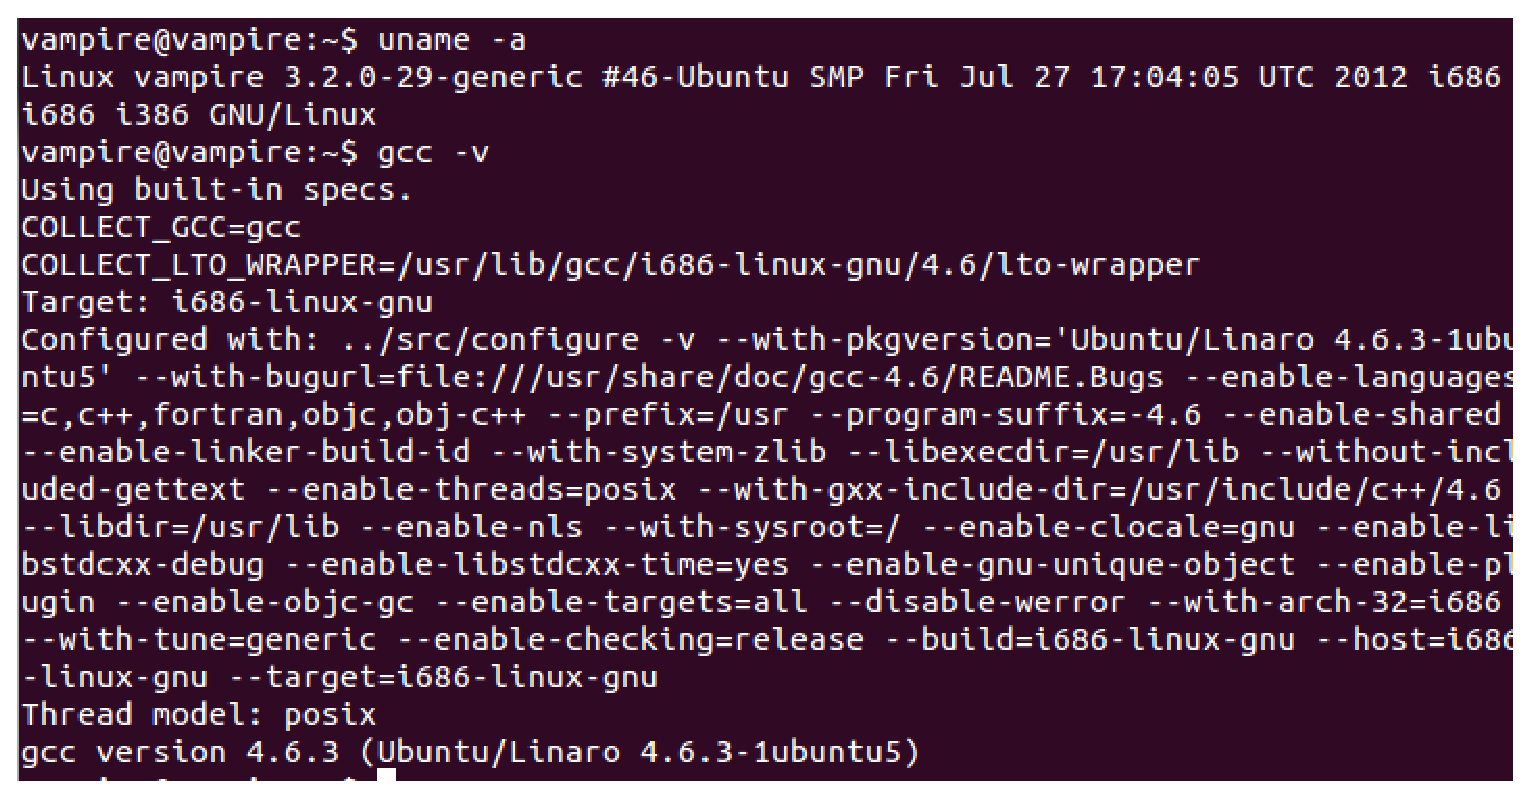
\includegraphics[width=0.90\textwidth]{env.eps}
  \caption{环境信息}
  \label{fig1}
\end{figure}

\subsection{代码分析}
代码\ref{lst1}和代码\ref{lst2}编译后的结果如下所示:
%\begin{singlespace}
\begin{parcolumenv}{1.0}
\begin{parcolumns}{2}
\colchunk[1]{\begin{acol}
push   %ebp
mov    %esp,%ebp
push   %edi
push   %ebx
sub    $0x410,%esp
mov    %gs:0x14,%eax
mov    %eax,-0xc(%ebp)
xor    %eax,%eax
lea    -0x40c(%ebp),%ebx

mov    $0x0,%eax
mov    $0x100,%edx
mov    %ebx,%edi
mov    %edx,%ecx
rep stos %eax,%es:(%edi)
mov    -0xc(%ebp),%eax
xor    %gs:0x14,%eax
je     8048441 <func+0x3d>
call   8048320 <__stack_chk_fail@plt>
add    $0x410,%esp
pop    %ebx
pop    %edi
pop    %ebp
ret    
\end{acol}}

\colchunk[2]{\begin{acol}
push   %ebp
mov    %esp,%ebp
push   %edi
push   %ebx
sub    $0x410,%esp
mov    %gs:0x14,%eax
mov    %eax,-0xc(%ebp)
xor    %eax,%eax
lea    -0x40c(%ebp),%eax
mov    %eax,%ebx
mov    $0x0,%eax
mov    $0x100,%edx
mov    %ebx,%edi
mov    %edx,%ecx
rep stos %eax,%es:(%edi)
mov    -0xc(%ebp),%eax
xor    %gs:0x14,%eax
je     8048443 <func+0x3f>
call   8048320 <__stack_chk_fail@plt>
add    $0x410,%esp
pop    %ebx
pop    %edi
pop    %ebp
ret    
\end{acol}}
\end{parcolumns}
\end{parcolumenv}
%\end{singlespace}
可以看出,编译后的两份代码只在第9、10行有一点差异\footnote{其实功能完全相同。},其余部分完全相同。而且还有一个明显的特点是:代码\ref{lst2}虽然调用了memset来初始化数组,但在编译后的代码里根本就没有调用memset来初始化\footnote{如果有调用的话,汇编代码里应该有一行call memset的指令。}。

既然代码一样,那我们只拿一份来分析说明,如下所示:
\lstinputlisting[label=lst3,language={[x86masm]Assembler}]{list/func.s}

第1和2行是每个函数开始执行的例行公事:保存上一个函数\footnote{调用该函数的函数,即调用者(caller)。}调用栈的栈基址,然后将本函数的栈基址保存到{\color{blue}\%ebp}寄存器,如图\ref{fig2}所示。与之对应的是第23和24行,首先将调用者的栈基址重新载入{\color{blue}\%ebp}寄存器,然后返回。

因为栈的操作基本都是基于栈基址\footnote{\%ebp寄存器的值。}偏移来实现的,所以调用者在调用一个函数的前后,其基址是不能改变的,但被调用者同样也会使用寄存器{\color{blue}\%ebp}来操作其堆栈,所以每个函数在使用{\color{blue}\%ebp}前,必需先保存寄存器的当前值,在返回前将其restore。
\begin{figure}[!htb]
  \setlength{\abovecaptionskip}{0pt}
  \begin{center}
    \begin{singlespace}
      \begin{tikzpicture}[auto,
        rect/.style={
          rectangle split, rectangle split parts=9,
          draw,rectangle split part align=center,draw, thick,
          text width=3cm,
          text centered, %minimum height=26em,
          align=center, rectangle split part align={center,left},
          rectangle split part align=midway,
          rectangle split part fill={gray!30, blue!20, blue!15, blue!20,blue!15,blue!15,green!15,green!20,green!30}
        }]

        % Split Rectangle
        \node (stack) [rect] {
          \nodepart {one} \Textbox{2.5cm}{$\rvdots$}
          \nodepart {two} \Textbox{1.0cm}{$\rvdots$}
          \nodepart{three} \Textbox{0.6cm}{Argument n}
          \nodepart{four} \Textbox{0.6cm}{$\rvdots$}
          \nodepart{five} \Textbox{0.6cm}{Argument 1}
          \nodepart{six} \Textbox{0.6cm}{Return Address}
          \nodepart{seven} \Textbox{0.6cm}{Saved \%ebp}
          \nodepart{eight} \Textbox{2.0cm}{Saved registers, local variables, and temporaries}
          \nodepart{nine} \Textbox{1.5cm}{Argument build area}
        };

        \draw [decorate,decoration={brace,amplitude=10pt}]
        (stack.north east) -- (stack.one split east) node [black,midway,xshift=0.3cm] 
        {\footnotesize $Earlier frames$};

        \draw [decorate,decoration={brace,amplitude=10pt}]
        (stack.one split east) -- (stack.six split east) node [black,midway,xshift=0.3cm] 
        {\footnotesize $Caller's frames$};

        \draw [decorate,decoration={brace,amplitude=10pt}]
        (stack.six split east) -- (stack.south east) node [black,midway,xshift=0.3cm] 
        {\footnotesize $Current frames$};

        \node[xshift=1pt,anchor=east] at (stack.three west) {\footnotesize $+4+4n$};
        \node[xshift=1pt,anchor=east] at (stack.five west) {\footnotesize $+8$};
        \node[xshift=1pt,anchor=east] at (stack.six west) {\footnotesize $+4$};
        \node[xshift=1pt,yshift=-10pt,anchor=east] at (stack.seven split west) {\footnotesize $-4$};

        \node[yshift=1pt,anchor=south] at (stack.north) {\footnotesize $Stack\ "bottom"$};
        \node[yshift=-1pt,anchor=north] at (stack.south) {\footnotesize $Stack\ "top"$};

        \draw [-latex,thick] ($(stack.four split west) + (-3,0)$) -- ($(stack.one split west) + (-3,2)$)
        node [draw=none,rotate=90,midway,above=0cm] {\footnotesize $Increasing\ address$};

        \draw [-latex,thick] ($(stack.seven west) + (-3,0)$) -- ($(stack.seven west) + (0,0)$)
        node [draw=none,midway,above=0cm] {\footnotesize $Frame\ pointer\ \%ebp$};

        \draw [-latex,thick] ($(stack.nine west) + (-3,-0.7)$) -- ($(stack.nine west) + (0,-0.7)$)
        node [draw=none,midway,above=0cm] {\footnotesize $Stack\ pointer\ \%esp$};

      \end{tikzpicture}
    \end{singlespace}
  \end{center}
  \label{fig2}
  \caption{函数调用栈}
\end{figure}

寄存器{\color{blue}\%edi}、{\color{blue}\%ebx}和{\color{blue}\%esi}是被调用者保存寄存器\footnote{与之对应的是调用者保存寄存器:\%eax、\%edx和\%ecx。},即如果当前函数需要使用这些寄存器,必须先将寄存器当前的内容压栈,然后在返回前restore。第3、4和第21、22行就是完成这个工作的。

第5行是为当前调用栈申请栈空间。紧拉着第6和7行是编译器为缓冲区保护自动插入的代码,其基本原理是:在栈的某个地址\footnote{该地址的值在函数正常执行的情况下不会被修改。}保存一个随机值,然后在函数返回前,查看该地址的值是否被修改,如果被修改,则说明栈被破坏了,直接抛出异常({\color{blue}17--19行})。

{\color{orange}紧接着8到15行就是对数组的初始化。第9行先将数组的首地址存到寄存器\%ebx中;接着第11行重置寄存器\%eax;第12行将数组的元素个数存入寄存器\%edx;第13、14行是将数组的元素个数存入寄存器\%ecx中,作为循环初始化数组的循环变量;最后第15行循环初始化数组,每次初始化4字节,一共循环256次直到寄存器\%ecx的值变为0。}

\subsection{循环还是memset}
从上一小节对编译后的代码分析可以知道,无论是memset还是\{0\},最终都是通过循环每次初始化4字节完成的。那是不是无论memset还是\{0\},最终都被编译成了每次4字节的循环初始化呢?让我们把代码\ref{lst1}和\ref{lst2}中的数组大小调整到10K看一下编译后的结果。如下所示:
\begin{parcolumenv}{1.0}
\begin{parcolumns}{2}
\colchunk[1]{\begin{acol}
push   %ebp
mov    %esp,%ebp
sub    $0x2828,%esp
mov    %gs:0x14,%eax
mov    %eax,-0xc(%ebp)
xor    %eax,%eax
lea    -0x280c(%ebp),%eax
mov    $0x2800,%edx
mov    %edx,0x8(%esp)
movl   $0x0,0x4(%esp)
mov    %eax,(%esp)
call   8048370 <memset@plt>
mov    -0xc(%ebp),%eax
xor    %gs:0x14,%eax
je     8048478 <func+0x44>
call   8048340 <__stack_chk_fail@plt>
leave  
ret 
\end{acol}}

\colchunk[2]{\begin{acol}
push   %ebp
mov    %esp,%ebp
sub    $0x2828,%esp
mov    %gs:0x14,%eax
mov    %eax,-0xc(%ebp)
xor    %eax,%eax
lea    -0x280c(%ebp),%eax
mov    $0x2800,%edx
mov    %edx,0x8(%esp)
movl   $0x0,0x4(%esp)
mov    %eax,(%esp)
call   8048370 <memset@plt>
mov    -0xc(%ebp),%eax
xor    %gs:0x14,%eax
je     8048478 <func+0x44>
call   8048340 <__stack_chk_fail@plt>
leave  
ret   
\end{acol}}
\end{parcolumns}
\end{parcolumenv}
可以看出,调整大小后的数组,无论是memset还是\{0\}初始化,最终都是通过调用memset完成的。网上查了一些资料,原来这是编译器的优化策略,对于小数组,直接循环初始化,大数组使用memset初始化。那数组达到多大的时候编译器会自动使用memset呢?在我的机子上测试的结果是大于8K,但在公司的单板服务器上测的结果是大于64个字节。这可能跟编译器版本及平台有关,这里不再继续深入分析。

\section{结论}
数组初始化,memset和\{0\}完全等价。

\end{document}
%%%%%%%%%%%%%%%%%%%%%%%%% 正文部分结束%%%%%%%%%%%%%%%%%%%%%%

